%!TEX options = --shell-escape


\documentclass[doctor]{thesis-uestc}


\title{XXXXXXXXXXXX\\XXXXXXXXX}
\englishtitle{XXXXXXXXXXXXXXXXXX}
\author{XXXXXX}
\englishauthor{XXXXXX}
\advisor{XXX\chinesespace 教授}
\englishadvisor{Prof. XXX}
\school{XXXXXX}
\englishschool{XXXXXX}
\major{XXXXXX}
\englishmajor{XXXXXXXXXXXX}
\studentid{XXXXXXXXXXXX}

\begin{document}

\makecover

% this is a thesis template with mutiple files: the chapters and the misc in standalone mode
% to avoid too many files in current folder, template add extra direcotry: chapter and misc
% please do not change the sequence of each one except the chapters themselves.
% by FengYouzheng.
% In fact, you have to alter several settings, including but not limit to, the cover, the layout and the style of the manuscript, so as to fit for the requirements of uestc thesis. So good luck.
% by Zhiyuan Ma.

% abstract
\documentclass{standalone}
% preamble: usepackage, etc.
\begin{document}
	
\begin{chineseabstract}

为了适应日益增长的宽带信号和非线性系统的工程应用,用于分析瞬态电磁散射问题的时域积分方程方法研究日趋活跃。本文以时域积分方程时间步进算法及其快速算法为研究课题,重点研究了时间步进算法的数值实现技术、后时稳定性问题以及两层平面波算法加速计算等,主要研究内容分为四部分。

针对这些问题,论文围绕XXXXXX展开研究,取得了如下研究成果:
%enumerate的设置参考https://blog.csdn.net/hu3350261/article/details/77451008
%其中的数值是试出来的。
\begin{enumerate}[labelsep = .5em, leftmargin = 0pt, itemindent = 3.8em]
%这个不能作为主要研究内容,最好作为
\item[(1)]
研究成果1的描述。
\item[(2)]
研究成果2的描述。
\item[(3)]
研究成果3的描述。
\end{enumerate}

\chinesekeyword{时域电磁散射,时域积分方程,时间步进算法,后时不稳定性,时域平面波算法}
\end{chineseabstract}

\end{document}
\documentclass{standalone}
% preamble: usepackage, etc.
\begin{document}

\begin{englishabstract}
	With the widespread engineering applications ranging from broadband signals and non-linear systems, time-domain integral equations (TDIE) methods for analyzing transient electromagnetic scattering problems are becoming widely used nowadays. TDIE-based marching-on-in-time (MOT) scheme and its fast algorithm are researched in this dissertation, including the numerical techniques of MOT scheme, late-time stability of MOT scheme, and two-level PWTD-enhanced MOT scheme. The contents are divided into four parts shown as follows.
	
	
	Aiming at these problems, the thesis focuses on XXXXXX, and achieves the following research results:	
	\begin{enumerate}[labelsep = .5em, leftmargin = 0pt, itemindent = 3.8em]
	\item[(1)] 
	Descriptions on result 1.
	\item[(2)] 
	Description on result 2.
	\item[(3)] 
	Description on result 3.
	\end{enumerate}
	
	
	\englishkeyword{time-domain electromagnetic scattering, time-domain integral equation (TDIE), marching-on in-time (MOT) scheme, late-time instability, plane wave time-domain (PWTD) algorithm}
\end{englishabstract}

\end{document}

%为了方便打印,留出空白页的代码,其中的数字根据当前要保留的页码-2来设置
%{
%\clearpage
% \phantom{s}
% \thispagestyle{empty}
% \setcounter{page}{4}
%   \setcounter{pseudopage}{4}
% }
% table of contents
\thesistableofcontents
%图形目录,如果有的话,放这里
%\thesisfigurelist
%%表格目录,如果有的话,放这里
%\thesistablelist



%缩略词表,如果有的话,在这里
\documentclass{standalone}
% preamble: usepackage, etc.
\begin{document}

%\chapter*{缩略词表}
%\thispagestyle{fancy}
%    \fancyhead[C]{\fontsize{10.5pt}{12.6pt}\selectfont 缩略词表}
%\fancyfoot[CE,CO]{\fontsize{9pt}{10.8pt}\selectfont\Roman{pseudopage}}
%上面在设置格式
\begin{thesisabbr}
%\begin{table}[h]
%	\begin{tabular}{p{2 cm}p{8cm}p{4 cm}} 
{
\renewcommand{\arraystretch}{0.7}
%\xiaosihao
\begin{longtable}{p{2.3 cm}@{\hskip 5 pt}p{7.7cm}@{\hskip 5 pt}p{4.2 cm}} 	%总宽15cm
		\textbf{缩略词} & \textbf{英文全称} & \textbf{中文全称}\\
		TD & Target Domain & 目标领域 \\
		SD & Source Domain & 源领域 \\
\end{longtable}
%	\end{tabular}
%\end{table}
}

\end{thesisabbr}

\end{document}

%主要符号表,如果有的话,在这里
\documentclass{standalone}
% preamble: usepackage, etc.
\begin{document}

%\chapter*{主要符号表}
%\thispagestyle{fancy}
%    \fancyhead[C]{\fontsize{10.5pt}{12.6pt}\selectfont 主要符号表}
%\fancyfoot[CE,CO]{\fontsize{9pt}{10.8pt}\selectfont\Roman{pseudopage}}

\begin{thesissymbols}

{
\renewcommand{\arraystretch}{1}

\begin{table}[htb!]
	\begin{tabular}{>{\xiaosihao}p{2 cm}>{\xiaosihao}p{8cm}}	%按列调整字体大小
		\textbf{符号} & \textbf{说明} \\
		$R^{m \times n}$ & $m \times n$维的实数空间 \\
		$C^{m \times n}$ & $m \times n$维的复数空间	\\	
	\end{tabular}
\end{table}
}

\end{thesissymbols}

%奇数页的时候增加一页空白页
\clearpage
 \phantom{s}
 \thispagestyle{empty}
\end{document}

% thesis contents
\documentclass{standalone}
% preamble: usepackage, etc.
\begin{document}

\thesischapterexordium

\section{研究工作的背景与意义}

计算电磁学方法\citing{wang1999sanwei, liuxf2006, zhu1973wulixue, chen2001hao, gu2012lao, feng997he}从时、频域角度划分可以分为频域方法与时域方法两大类。频域方法的研究开展较早,目前应用广泛的包括:矩量法(MOM)\citing{xiao2012yi,zhong1994zhong}及其快速算法多层快速多极子(MLFMA)\citing{clerc2010discrete}方法、有限元(FEM)\citing{wang1999sanwei,zhu1973wulixue}方法、自适应积分(AIM)\citing{gu2012lao}方法等,这些方法是目前计算电磁学商用软件
\footnote{脚注序号“\ding{172},……,\ding{180}”的字体是“正文”,不是“上标”,序号与脚注内容文字之间空1个半角字符,脚注的段落格式为:单倍行距,段前空0磅,段后空0磅,悬挂缩进1.5字符;中文用宋体,字号为小五号,英文和数字用Times New Roman字体,字号为9磅;中英文混排时,所有标点符号(例如逗号“,”、括号“()”等)一律使用中文输入状态下的标点符号,但小数点采用英文状态下的样式“.”。}
(例如:FEKO、Ansys 等)的核心算法。

\section{时域积分方程方法的国内外研究历史与现状}
时域积分方程方法的研究始于上世纪60年代,C.L.Bennet等学者针对导体目标的瞬态电磁散射问题提出了求解时域积分方程的时间步进(marching-on in-time, MOT)算法[14]。

\section{本文的主要贡献与创新}

本论文以时域积分方程时间步进算法的数值实现技术、后时稳定性问题以及两层平面波加速算法为重点研究内容,主要创新点与贡献如下:

\section{本论文的结构安排}
介绍本文的组织结构,各章节之间的关系,尤其是后面涉及的应用领域的研究呈现出并列关系,

\end{document}
\documentclass{standalone}
% preamble: usepackage, etc.
\begin{document}

\chapter{时域积分方程基础}
时域积分方程(TDIE)方法作为分析瞬态电磁波动现象最主要的数值算法之一,常用于求解均匀散射体和表面散射体的瞬态电磁散射问题。

\section{时域积分方程的类型}

\section{空间基函数与时间基函数}
利用数值算法求解时域积分方程,首先需要选取适当的空间基函数与时间基
函数对待求感应电流进行离散。

\subsection{空间基函数}
RWG 基函数是定义在三角形单元上的最具代表性的基函数。它的具体定义如
下:
\begin{equation}
f_n(r)=
\begin{lcase}
&\frac{l_n}{2A_n^+}\rho_n^+=\frac{l_n}{2A_n^+}(r-r_+)&r\in T_n^+\\
&\frac{l_n}{2A_n^-}\rho_n^-=\frac{l_n}{2A_n^-}(r_--r)&r\in T_n^-\\
& 0  &\text{otherwise}
\end{lcase}
\end{equation}

其中,$l_n$为三角形单元$T_n^+$和$T_n^-$公共边的长度,$A_n^+$和$A_n^-$分别为三角形单元$T_n^+$和$T_n^-$的面积(如图\ref{pica}所示)。

\begin{figure}[h]
	\includegraphics{pica.pdf}
	\caption{RWG 基函数几何参数示意图}
	\label{pica}
\end{figure}
由于时域混合场积分方程是时域电场积分方程与时域磁场积分方程的线性组合,因此时域混合场积分方程时间步进算法的阻抗矩阵特征与时域电场积分方程时间步进算法的阻抗矩阵特征相同。
\begin{equation}
\label{latent_binary_variable}
\mathbf{r}_{i,j}=
\begin{lcase}
& 1,f(\mathbf{x}^{i};\mathbf{w})\cdot f(\mathbf{x}^{j};\mathbf{w})\geq u(\lambda),\\
& 0,f(\mathbf{x}^{i};\mathbf{w})\cdot f(\mathbf{x}^{j};\mathbf{w})< l(\lambda), 1\leq i,j\leq n.\\
& f(\mathbf{x}^{i};\mathbf{w})\cdot f(\mathbf{x}^{j};\mathbf{w}),\text{otherwise},
\end{lcase}
\end{equation}

时域积分方程时间步进算法的阻抗元素直接影响算法的后时稳定性,因此阻抗元素的计算是算法的关键之一,采用精度高效的方法计算时域阻抗元素是时域积分方程时间步进算法研究的重点之一。


\subsection{时间基函数}

\subsubsection{时域方法特有的展开函数}

\subsubsection{频域方法特有的展开函数}

\section{入射波}

如图\ref{picb}和图\ref{picc}所示分别给出了参数$E_0=\hat{x}$,$a_n=-\hat{z}$,$f_0=250MHz$,$f_w=50MHz$,$t_w=4.2\sigma$时,调制高斯脉冲的时域与频域归一化波形图。

\begin{figure}[h]
	\subfigure[]{
		\label{picb}
		\includegraphics[width=7.3cm]{picb.pdf}}
	\subfigure[]{
		\label{picc}
		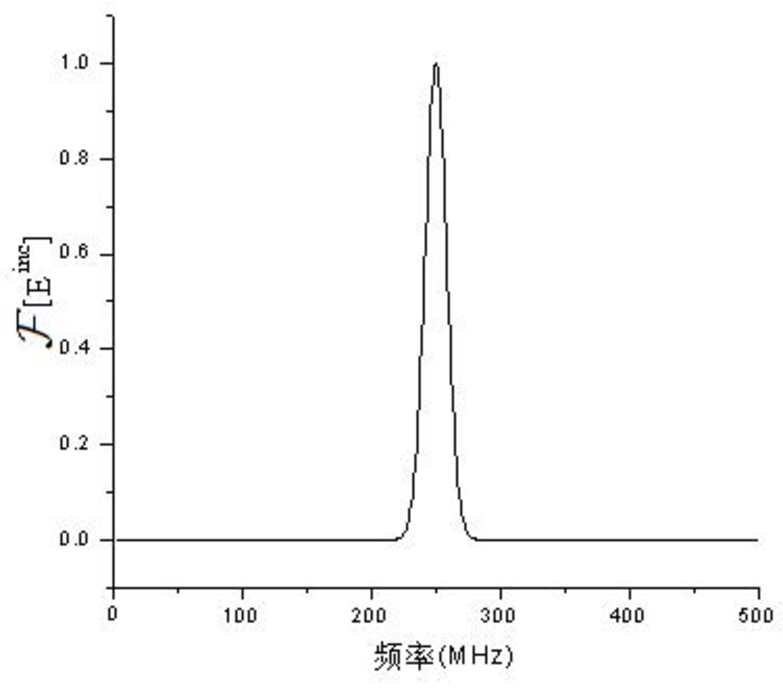
\includegraphics[width=6.41cm]{picc.pdf}}
	\caption{调制高斯脉冲时域与频率波形,时域阻抗元素的存储技术也是时间步进算法并行化的关键技术之一,采用合适的阻抗元素存储方式可以很大的提高并行时间步进算法的计算效率。}
	\label{fig1}
\end{figure}
时域阻抗元素的存储技术\citing{xiao2012yi}也是时间步进算法并行化的关键技术之一,采用合适的阻抗元素存储方式可以很大的提高并行时间步进算法的计算效率。

\section{本章小结}
本章首先从时域麦克斯韦方程组出发推导得到了时域电场、磁场以及混合场积分方程。

\chapter{时域积分方程数值方法研究}
\section{时域积分方程时间步进算法的阻抗元素精确计算}
时域积分方程时间步进算法的阻抗元素直接影响算法的后时稳定性,因此阻抗元素的计算是算法的关键之一,采用精度高效的方法计算时域阻抗元素是时域积分方程时间步进算法研究的重点之一。

\section{时域积分方程时间步进算法阻抗矩阵的存储}
时域阻抗元素的存储技术也是时间步进算法并行化的关键技术之一,采用合适的阻抗元素存储方式可以很大的提高并行时间步进算法的计算效率。

\subsection{时域积分方程时间步进算法产生的阻抗矩阵的特征}
由于时域混合场积分方程是时域电场积分方程与时域磁场积分方程的线性组合,因此时域混合场积分方程时间步进算法的阻抗矩阵特征与时域电场积分方程时间步进算法的阻抗矩阵特征相同。

\subsection{数值算例与分析}

如图\ref{fig:subfig:VSbatch2}所示给出了时间步长选取为0.5ns时采用三种不同存储方式计算的平板中心处 方向的感应电流值与IDFT方法计算结果的比较。如图\ref{fig:subfig:VSbatch3}所示给出了存储方式为基权函数压缩存储方式,时间步长分别取时平板中心处 方向的感应电流计算结果,从图中可以看出不同时间步长的计算结果基本相同。

\begin{figure}[htb!]
%\setlength{\textwidth}{15.5 cm}
\centering
\subfigure[]{
\begin{minipage}[b]{0.45\textwidth}
\centering
\includegraphics[width=1\textwidth,height=3cm]{figures/pica.pdf} \\
\label{fig:subfig:VSbatch2}
\vspace{-5 pt}
\end{minipage}
}
\vspace{-6 pt}
\subfigure[]{
\begin{minipage}[b]{0.45\textwidth}
\centering
\includegraphics[width=1\textwidth,height=3cm]{figures/picb.pdf} \\
\label{fig:subfig:VSbatch3}
\vspace{-5 pt}
\end{minipage}
}
\vspace{5 pt}
\caption{感应电流计算结果。\subref{fig:subfig:VSbatch2}感应电流值与IDFT方法计算结果;\subref{fig:subfig:VSbatch3}感应电流计算结果率}
\label{fig:DAELM_WDTELM_100}
\end{figure}

由于时域混合场积分方程是时域电场积分方程与时域磁场积分方程的线性组合,因此时域混合场积分方程时间步进算法的阻抗矩阵特征与时域电场积分方程时间步进算法的阻抗矩阵特征相同。



\section{本章小结}
本章首先研究了时域积分方程时间步进算法的阻抗元素精确计算技术,分别采用DUFFY变换法与卷积积分精度计算法计算时域阻抗元素,通过算例验证了计算方法的高精度。

\end{document}
\documentclass{standalone}
% preamble: usepackage, etc.
\begin{document}

\chapter{毕业论文其他格式参考}

由于时域混合场积分方程是时域电场积分方程与时域磁场积分方程的线性组
合,因此时域混合场积分方程时间步进算法的阻抗矩阵特征与时域电场积分方程
时间步进算法的阻抗矩阵特征相同。

\section{如何撰写公式}

行内公式可以参考这样的形式$O(n_1 \cdot (n_1 + m))$。如果需要对公式进行编号,可以参考公式(\ref{equ:4-1})。
\begin{equation}
\label{equ:4-1}
\begin{aligned}
\beta_i^{j} &=H_i^T K_{k}^{-1} (K_k^{-1} +C_{m} \delta h^T \delta h) \\
\end{aligned}
\end{equation}

跨行的公式可以参考公式(\ref{equ:4-2})。
\begin{equation}
\label{equ:4-2}
\begin{aligned}
\beta_i^{j} &=H_i^T K_{k}^{-1} (K_k^{-1} +C_{m} \delta h^T \delta h) \\
& =H_i^T K_{k}^{-1} (K_k^{-1} +C_{m} \delta h^T \delta h) \\
\end{aligned}
\end{equation}

向量的写法参考公式(\ref{equ:w-example})。
\begin{equation}
\label{equ:w-example}
\begin{aligned}
\renewcommand{\arraystretch}{0.5}
w_i=\begin{bmatrix}
\setlength{\parskip}{0 pt}
P_1 & P_2 & 0 & P_4 & 0 & 0
\end{bmatrix}
\end{aligned}
\end{equation}

\section{如何撰写一个枚举列表}

有时候需要撰写一个列表,列表的格式可以参考下面这种:
\begin{enumerate}[labelsep = .5em, leftmargin = 0pt, itemindent = 3.8em]
\item[(1)]描述1;
\item[(2)]描述2;
\item[(3)]描述3;
\item[(4)]重复(2)和(3)。
\end{enumerate}

\section{如何写一个大表格}

有时候表格的表头比较复杂,具体需要用到multirow和multicolumn这两个环境,写法可以参考表\ref{tab:Perf_XX}。

\begin{table}[h]
\caption{一个表格示例。}
\label{tab:Perf_XX}
\centering
%% \tablesize{} %% You can specify the fontsize here, e.g.  \tablesize{\footnotesize}. If commented out \small will be used.
\renewcommand{\arraystretch}{0.8}
\begin{tabular}{|c|c|c|c|c|c|c|c|}
\hline
\multicolumn{1}{|c|}{\multirow{1}{*}{XX}} &
\multicolumn{7}{c|}{XXXXXX} \\
%\multicolumn{7}{c}{\multirow{2}{*}{\textbf{Accuracy (\%)}} \\
\cline{2-8}
\multicolumn{1}{|c|}{\multirow{1}{*}{XX}}
	& \text{XX}	& \text{XX} & \text{XX} & \text{XX} & \text{XX} & \text{XX} & \text{XX}
\\
\hline
XX	& XX	& XX  & XX & XX & XX & XX &  XX\\
\hline
XX	& XX	& XX  & XX & XX & XX & XX &  XX\\
\hline
XX	& XX	& XX  & XX & XX & XX & XX &  XX\\
\hline
XX	& XX	& XX  & XX & XX & XX & XX &  XX\\
\hline
XX	& XX	& XX  & XX & XX & XX & XX &  XX\\
\hline
\end{tabular}
\end{table}

\section{如何写一个算法伪代码}

原模板没有如何写伪代码,这里提供一个例子,如算法\ref{alg:Ch2_template}。
需要注意的是,算法格式不跨行显示,所以需要根据大小调整在文中的位置。建议写完后根据文字占页情况调整下相应的位置。
\vspace{-5 pt}
\begin{algorithm}[htb!]
\caption{如何写一个算法}
\begin{algorithmic}[1]
\REQUIRE ~~\\
$data:=$输入数据;\\
\ENSURE ~~\\ %算法的输出:Output
$Out:=$输出数据;\\
\STATE Initialization初始化;
\FOR{for循环的条件}
\IF {if的条件判断句,例如$| data |<k$}
\STATE If语句中需要执行的程序;\\
\ELSE
\STATE	例外情况需要执行的语句;\\
\WHILE{while循环的判断条件}
\STATE	whil循环的操作; \\
\ENDWHILE
\ENDIF
\ENDFOR
\RETURN $Out$; \\%算法的返回值
\end{algorithmic}
\label{alg:Ch2_template}
\end{algorithm}

\section{本章小结}
本章首先研究了时域积分方程时间步进算法的阻抗元素精确计算技术,分别采用DUFFY变换法与卷积积分精度计算法计算时域阻抗元素,通过算例验证了计算方法的高精度。

\end{document}
\documentclass{standalone}
% preamble: usepackage, etc.
\begin{document}

\chapter{时域积分方程数值方法研究}
\section{时域积分方程时间步进算法的阻抗元素精确计算}
时域积分方程时间步进算法的阻抗元素直接影响算法的后时稳定性,因此阻
抗元素的计算是算法的关键之一,采用精度高效的方法计算时域阻抗元素是时域
积分方程时间步进算法研究的重点之一。

\section{时域积分方程时间步进算法阻抗矩阵的存储}
时域阻抗元素的存储技术也是时间步进算法并行化的关键技术之一,采用
合适的阻抗元素存储方式可以很大的提高并行时间步进算法的计算效率。

\subsection{时域积分方程时间步进算法产生的阻抗矩阵的特征}

由于时域混合场积分方程是时域电场积分方程与时域磁场积分方程的线性组
合,因此时域混合场积分方程时间步进算法的阻抗矩阵特征与时域电场积分方程
时间步进算法的阻抗矩阵特征相同。
\subsection{数值算例与分析}
如表\ref{tablea}所示给出了时间步长分别取0.4ns、0.5ns、0.6ns 时的三种存储
方式的存储量大小。

\begin{table}[h]
	\caption{计算$2m\times 2m$理想导体平板时域感应电流采用的三种存储方式的存储量比较。} 
	\begin{tabular}{|c|c|c|c|} 
		\hline  
		时间步长 & 非压缩存储方式 & 完全压缩存储方式 & 基权函数压缩存储方式 \\
		\hline 
		0.4ns & 5.59 MB & 6.78 MB & 6.78 MB\\  
		\hline  
		0.5ns & 10.17 MB & 5.58 MB & 5.58 MB \\  
		\hline  
		0.6ns & 8.38MB & 4.98 MB & 4.98 MB \\  
		\hline  
	\end{tabular}
	\label{tablea}
\end{table}

如图\ref{picd}所示给出了时间步长选取为0.5ns 时采用三种不同存储方式计算的
平板中心处$x$方向的感应电流值与IDFT 方法计算结果的比较,……。如图\ref{pice}
所示给出了存储方式为基权函数压缩存储方式,时间步长分别取0.4ns、0.5ns、0.6ns
时平板中心处$x$方向的感应电流计算结果,从图中可以看出不同时间步长的计算结果基本相同。

由于时域混合场积分方程是时域电场积分方程与时域磁场积分方程的线性组合,因此时域混合场积分方程时间步进算法的阻抗矩阵特征与时域电场积分方程时间步进算法的阻抗矩阵特征相同。

\begin{figure}[h]
	\subfigure[]{
		\label{picd}
		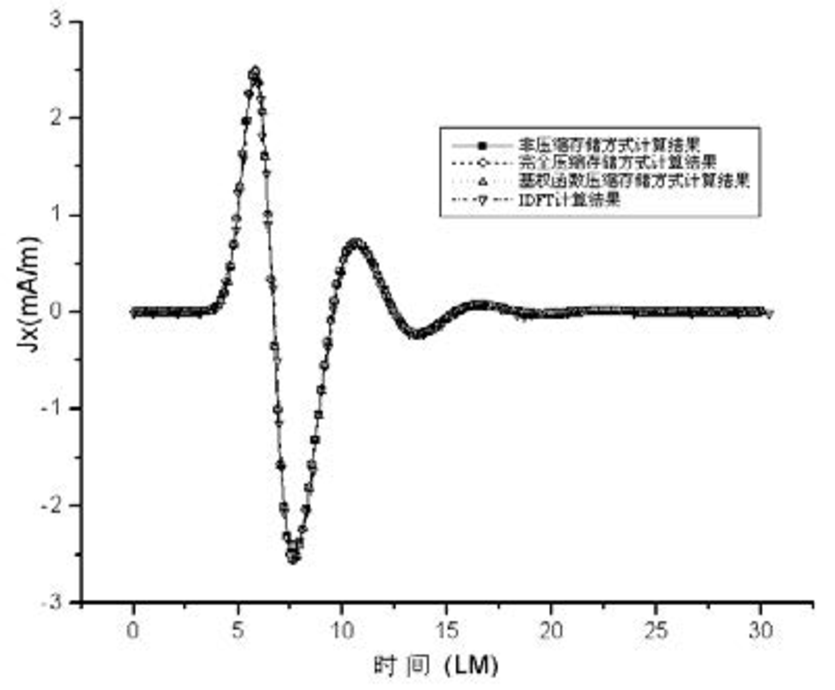
\includegraphics[width=6.77cm]{picd.pdf}}
	\subfigure[]{
		\label{pice}
		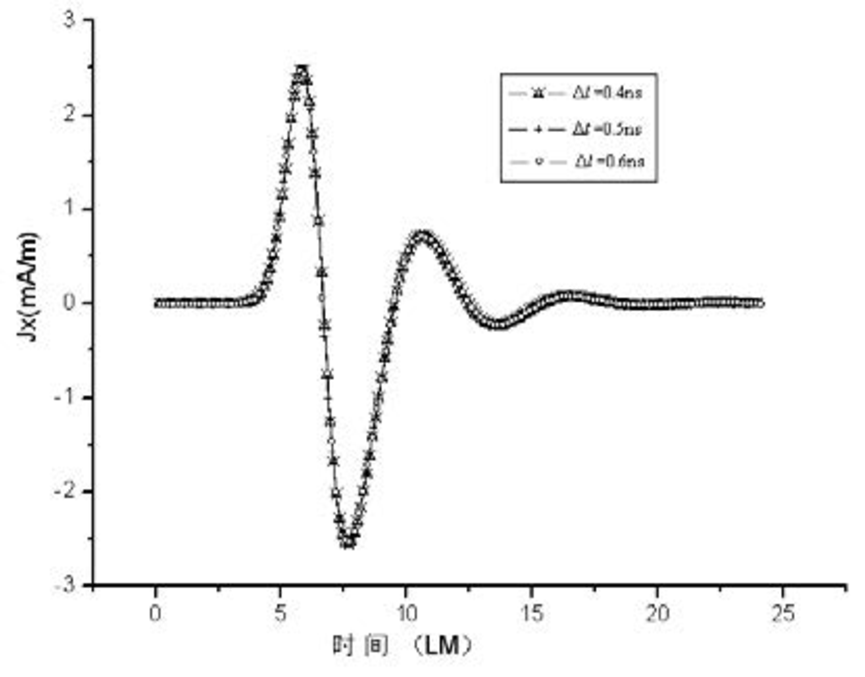
\includegraphics[width=7.04cm]{pice.pdf}}
	\caption{$2m\times 2m$的理想导体平板中心处感应电流$x$分量随时间的变化关系}
	\label{fig2}
\end{figure}


由于时域混合场积分方程是时域电场积分方程与时域磁场积分方程的线性组
合,因此时域混合场积分方程时间步进算法的阻抗矩阵特征与时域电场积分方程
时间步进算法的阻抗矩阵特征相同。
\section{时域积分方程时间步进算法矩阵方程的求解}

\begin{theorem}
	如果时域混合场积分方程是时域电场积分方程与时域磁场积分方程
	的线性组合。
\end{theorem}
\begin{proof}
	由于时域混合场积分方程是时域电场积分方程与时域磁场积分方程的线性组
	合,因此时域混合场积分方程时间步进算法的阻抗矩阵特征与时域电场积分方程
	时间步进算法的阻抗矩阵特征相同。
\end{proof}
\begin{corollary}
	时域积分方程方法的研究近几年发展迅速,在本文研究工作的基础上,仍有以下方向值得进一步研究。
\end{corollary}
\begin{lemma}
	因此时域混合场积分方程时间步进算法的阻抗矩阵特征与时域电场积分方程
	时间步进算法的阻抗矩阵特征相同。
\end{lemma}

\section{本章小结}
本章首先研究了时域积分方程时间步进算法的阻抗元素精确计算技术,分别
采用DUFFY 变换法与卷积积分精度计算法计算时域阻抗元素,通过算例验证了计
算方法的高精度。

\end{document}
\documentclass{standalone}
% preamble: usepackage, etc.
\begin{document}
	
\chapter{全文总结与展望}

\section{全文总结}
本文以时域积分方程方法为研究背景,主要对求解时域积分方程的时间步进算法以及两层平面波快速算法进行了研究。

\section{后续工作展望}
时域积分方程方法的研究近几年发展迅速,在本文研究工作的基础上,仍有以下方向值得进一步研究:

\end{document}


% misc
\documentclass{standalone}
% preamble: usepackage, etc.
\begin{document}

\thesisacknowledgement

艰难苦恨繁霜鬓,潦倒新停浊酒杯!


\end{document}
\thesisloadbibliography[nocite]{reference}

%
% Uncomment following codes to load bibliography database with native
% \bibliography command.
%
% \nocite{*}
% \bibliographystyle{thesis-uestc}
% \bibliography{reference}
%

% comment while no need
%\documentclass{standalone}
% preamble: usepackage, etc.
\usepackage{ulem}
\begin{document}

\thesisappendix

\section{}
\begin{lemma}
\label{lem:Inverse}
If $C_T,C_{Tu}>0$, $H_T \in R^{n_1*l}$ and $H_{Tu} \in R^{n_2 * l}$ are any arbitrary matrices defined in the paper, then $I+C_T P + C_{Tu} P^{-1}H_T H_{Tu}^T H_{Tu} H_T^T$ has inverse where $P=H_T H_T^T$.
\end{lemma}
\begin{proof}
Let $A$ be defined as $A=I+C_T P + C_{Tu} P^{-1}H_T H_{Tu}^T H_{Tu} H_T^T$. Consider a sequence of rank-one updates of $A$ as $A_k=I+C_T P + C_{Tu} P^{-1}H_T (\sum_{i=0}^{k}h_i^T h_i) H_T^T$ where $h_i \in R^{1*l}$ is the $i$th row of $H_{Tu}$. If we can prove $A_k$ has inverse for any arbitrary column vector $h_i$, \ref{lem:Inverse} is proved.

Let $A_k$ be written as (\ref{equ:ak}). Let $c_k=C_{Tu} P^{-1}H_T h_i$ and $d_k^T =h_i H_T^T$. Based on generalized inverse theory \cite{Campbell2009GENERALIZED}, the generalized inverse of $A_k$ has a unique form as (\ref{equ:ak_ginverse}) if $A_{k-1}$ has inverse and (\ref{equ:sequenceproof}) satisfies. It is easy to verify that, in this case, the generalized inverse of $A_{k-1}$ is the inverse. 
\begin{equation}
\label{equ:ak}
A_k=A_{k-1}+C_{Tu} P^{-1}H_T h_i^T h_i H_T^T
\end{equation}

\begin{equation}
\label{equ:ak_ginverse}
\begin{aligned}
A_k^{\dagger}&=A_{k-1}^{-1}-\frac{A_{k-1}^{-1}c_k d_k^T A_{k-1}^{-1}}{1+ d_k^T A_{k-1}c_k} 
\end{aligned}
\end{equation}

\begin{equation}
\label{equ:sequenceproof}
\begin{aligned}
%&A_{k-1}^{-1} \  exists, \\
&1+d_k^T A_{k-1}^{-1} c_k \ne 0.
\end{aligned}
\end{equation}

Therefore, the problem becomes proving that $A_{k-1}$ has inverse and (\ref{equ:sequenceproof}) stands. To achieve the goal, we can prove a stronger case as (\ref{equ:secondlemma}). 
\begin{equation}
\label{equ:secondlemma}
\begin{aligned}
d_k^T A_{k-1}^{-1} c_k \ge 0 \quad if \ A_{k-1}^{-1} \  exist
\end{aligned}
\end{equation}

Let $A_0=I+C_T H_T H_T^T$ and $h$ be an arbitrary row of $H_{Tu}$. Note that $C_T >0$, so $A_{0}$ has inverse. Based on Woodbury's formula, we can write $A_0^{-1}$ as (\ref{equ:a0_inverse}).
\begin{equation}
\label{equ:a0_inverse}
\begin{aligned}
A_0^{-1}=I - C_T H_T (I+ C_T H_T^T H_T)^{-1}H_T^T
\end{aligned}
\end{equation}

Let $A_1=A_0+c_1 d_1^T $ where $c_1=C_{Tu}P^{-1} H_T h^T$ and $d_1^T=h H_T^T$. Subsequently, we can write $d_1^T A_0^{-1}c_1$ as (\ref{equ:inver_a0}) by using Woodbury's formula. Note that $C_T H_T^T H_T$ is a positive semi-definite, so it is unitarily similar to a diagonal matrix, i.e. $H_T^T H_T=U diag(\epsilon_1,\epsilon_2,...,\epsilon_y) U^T$ where $\epsilon_1> \epsilon_2>...>\epsilon_y>0$. Similarly, $I+C_T H_T H_T^T$ is unitarily similar to a diagonal matrix, i.e. $I+C_T H_T H_T^T=U diag(1+C_T \epsilon_1, 1+C_T \epsilon_2,...,1+C_T \epsilon_y)U^T$. Note that they share the same $U$, therefore $d_1^T A_0^{-1}c_1 \ge 0$ stands. Consequently, $A_1$ has inverse.
\begin{equation}
\label{equ:inver_a0}
\begin{aligned}
d_1^T A_0^{-1}c_1 &= h H_T^T A_0^{-1} C_{Tu} P^{-1}H_T h^T \\
&=C_{Tu} h H_T^T (I- C_T H_T (I+ C_T H_T^T H_T)^{-1} H_T^T)  P^{-1} H_T h^T \\
&=C_{Tu} h(I-C_T H_T^T H_T (I+ C_T H_T^T H_T)^{-1})H_T^T P^{-1}H_T h^T \\
&=C_{Tu} h (I-C_T H_T^T H_T)^{-1} H_T^T P^{-1}H_T h^T \\
&=C_{Tu} h (I-C_T H_T^T (I+C_T H_T H_T^T)^{-1} H_T)H_T^T P^{-1} H_T h \\
&=C_{Tu} h H_T^T (P^{-1}-C_T (I+ C_T H_T H_T^T)^{-1})H_T h^T \\
&=C_{Tu} h H_T^T P^{-1}(I+C_T H_T H_T^T)^{-1}H_Th^T \\
&=C_{Tu} h H_T^T P^{-1} A_0^{-1} H_T h^T \\
\end{aligned}
\end{equation}

Based on (\ref{equ:inver_a0}), we can further define (\ref{equ:beta_0}) which is inversible.
\begin{equation}
\label{equ:beta_0}
\begin{aligned}
B_0 &= A_0^{-1} P^{-1}
\end{aligned}
\end{equation}

Assume $A_k$ has inverse. By using Woodbury's formula, we can write $A_k^{-1}$ as (\ref{equ:a_k}).
\begin{equation}
\label{equ:a_k}
\begin{aligned}
A_k^{-1} & = (A_0 + C_{Tu} P^{-1} H_T H_{Tu}^T H_{Tu} H_T)^{-1} \\
&= A_0^{-1} -C_{Tu} A_0^{-1} P^{-1} H_T H_{Tu}^T  (I+ C_{Tu} H_{Tu} B_0 H_{Tu}^T)^{-1} H_{Tu} H_T^T A_0^{-1} \\
\end{aligned}
\end{equation}

For the case of $A_{k+1}=A_k +C_{Tu}P^{-1}H_T h^T h H_T^T$ where $h$ is an arbitrary row of $H_{Tu}$, we can combine (\ref{equ:beta_0}) and (\ref{equ:a_k}) to write $d_{k+1}^T A_k^{-1} c_{k+1}$ as (\ref{equ:A_k1_def}) where $c_{k+1}=C_{Tu} P^{-1}H_T h^T \in R^{n_1*1}$ and $d_{k+1}^T = h H_T^T \in R^{1*n_1}$. Note that $h$ is an arbitrary row of $H_{Tu}$. Similarly, we have $d_{k+1}^T A_k^{-1} c_{k+1} \ge 0$ stands.

\begin{equation}
\label{equ:A_k1_def}
\begin{aligned}
 d_{k+1}^T A_k^{-1} c_{k+1} &= C_{Tu} h H_T^T(B_0 - C_{Tu} B_0 H_{Tu}^T (I +  C_{Tu} H_{Tu} B_0  H_{Tu}^T)^{-1} H_{Tu} B_0)H_T h^T \\
&=C_{Tu} h (B_0^{-1}+C_{Tu} H_{Tu}^T H_{Tu})^{-1} h^T \\
\end{aligned}
\end{equation}

By using mathematical induction, we can prove that $d_{k}^T A_{k-1}^{-1} c_{k} \ge 0$ stands for any $k$. Subsequently, $A_k$ has inverse for any $k$. To sum up, Lemma \ref{lem:Inverse} has been proved.
\end{proof}

\end{document}
%\thesisloadachievement{publications} %这个少了一些定义,所以用不了。

\begin{thesisachievement}
\setlength{\baselineskip}{20 pt}	%调整下行间距
\addtolength{\itemsep}{-2 ex}	%用来调整行间距,默认会空一行,有时候太长了
\section*{发表论文}
\bibitem{1}
\textbf{X. XX}, X. XX, X. XX. XXXXXXXXXXXXX[J]. XXXXXXXXXX, 2018, 2018:1-17(SCI,IF X.XXX)
\bibitem{2}
\textbf{X. XX}, X. XX, X. XX. XXXXXXXXXXXXX[J]. XXXXXXXXXX, 2018, 2018:1-17(SCI,IF X.XXX)
\vspace{-5 pt}	%调整间距
\section*{著作}
写自己的著作
\section*{主研/参研项目}
\bibitem[1]{1} 参与,编号:XXXXXXXXXX,四川省科技厅,XXXXXXXXX
\bibitem[2]{2} 参与,编号:XXXXXXXXXX,四川省科技厅,XXXXXXXXX
\bibitem[3]{3} 参与,编号:XXXXXXXXXX,四川省科技厅,XXXXXXXXX


%[M]John Wiley \& Sons,2017, 163-210

\end{thesisachievement}

%\documentclass{standalone}
% preamble: usepackage, etc.
\begin{document}

\thesistranslationoriginal
\section{A Tight Upper Bound on Bit Error Rate}

\end{document}
%\documentclass{standalone}
% preamble: usepackage, etc.
\begin{document}

\thesistranslationchinese
\section{基于多载波索引键控的正交频分多路复用系统模型}

\end{document}

\end{document}
